%%%%%%%%%%%%%%%%%%%%%%%%%%%%%%%%%%%%%%%%%%%%%%%%%%%%%%%%%%%%%%%%%%%%%%%%%%%%%%%%%%%%%%%%%%
% Ceci est le fichier principal du template template à utiliser pour les rapports du     %
% projet 1 (Construction de Programme) d'INFO0947.                                       %
%                                                                                        %
% Vous devez décommenter et compléter les commandes introduites plus bas (intitule, ...) %
% avant de pouvoir compiler le fichier LaTeX.  Pensez à configurer votre Makefile en     %
% conséquence.                                                                           %
%                                                                                        %
% Le contenu et la structure du rapport sont imposés.  Vous devez compléter les          %
% différents fichiers .tex inclus dans ce fichier avec votre production.                 %
%%%%%%%%%%%%%%%%%%%%%%%%%%%%%%%%%%%%%%%%%%%%%%%%%%%%%%%%%%%%%%%%%%%%%%%%%%%%%%%%%%%%%%%%%%

% !TEX root = ./main.tex
% !TEX engine = latexmk -pdf
% !TEX buildOnSave = true
\documentclass[a4paper, 11pt, oneside]{article}

\usepackage[utf8]{inputenc}
\usepackage[T1]{fontenc}
\usepackage[french]{babel}
\usepackage{array}
\usepackage{shortvrb}
\usepackage{listings}
\usepackage[fleqn]{amsmath}
\usepackage{amsfonts}
\usepackage{fullpage}
\usepackage{enumerate}
\usepackage{graphicx}             % import, scale, and rotate graphics
\usepackage{subfigure}            % group figures
\usepackage{alltt}
\usepackage{url}
\usepackage{indentfirst}
\usepackage{eurosym}
\usepackage{listings}
\usepackage{color}
\usepackage[table,xcdraw,dvipsnames]{xcolor}

% Change le nom par défaut des listing
\renewcommand{\lstlistingname}{Extrait de Code}


\definecolor{mygray}{rgb}{0.5,0.5,0.5}
\newcommand{\coms}[1]{\textcolor{MidnightBlue}{#1}}

\lstset{
    language=C, % Utilisation du langage C
    commentstyle={\color{MidnightBlue}}, % Couleur des commentaires
    frame=single, % Entoure le code d'un joli cadre
    rulecolor=\color{black}, % Couleur de la ligne qui forme le cadre
    stringstyle=\color{RawSienna}, % Couleur des chaines de caractères
    numbers=left, % Ajoute une numérotation des lignes à gauche
    numbersep=5pt, % Distance entre les numérots de lignes et le code
    numberstyle=\tiny\color{mygray}, % Couleur des numéros de lignes
    basicstyle=\tt\footnotesize,
    tabsize=3, % Largeur des tabulations par défaut
    keywordstyle=\tt\bf\footnotesize\color{Sepia}, % Style des mots-clés
    extendedchars=true,
    captionpos=b, % sets the caption-position to bottom
    texcl=true, % Commentaires sur une ligne interprétés en Latex
    showstringspaces=false, % Ne montre pas les espace dans les chaines de caractères
    escapeinside={(>}{<)}, % Permet de mettre du latex entre des <( et )>.
    inputencoding=utf8,
    literate=
  {á}{{\'a}}1 {é}{{\'e}}1 {í}{{\'i}}1 {ó}{{\'o}}1 {ú}{{\'u}}1
  {Á}{{\'A}}1 {É}{{\'E}}1 {Í}{{\'I}}1 {Ó}{{\'O}}1 {Ú}{{\'U}}1
  {à}{{\`a}}1 {è}{{\`e}}1 {ì}{{\`i}}1 {ò}{{\`o}}1 {ù}{{\`u}}1
  {À}{{\`A}}1 {È}{{\`E}}1 {Ì}{{\`I}}1 {Ò}{{\`O}}1 {Ù}{{\`U}}1
  {ä}{{\"a}}1 {ë}{{\"e}}1 {ï}{{\"i}}1 {ö}{{\"o}}1 {ü}{{\"u}}1
  {Ä}{{\"A}}1 {Ë}{{\"E}}1 {Ï}{{\"I}}1 {Ö}{{\"O}}1 {Ü}{{\"U}}1
  {â}{{\^a}}1 {ê}{{\^e}}1 {î}{{\^i}}1 {ô}{{\^o}}1 {û}{{\^u}}1
  {Â}{{\^A}}1 {Ê}{{\^E}}1 {Î}{{\^I}}1 {Ô}{{\^O}}1 {Û}{{\^U}}1
  {œ}{{\oe}}1 {Œ}{{\OE}}1 {æ}{{\ae}}1 {Æ}{{\AE}}1 {ß}{{\ss}}1
  {ű}{{\H{u}}}1 {Ű}{{\H{U}}}1 {ő}{{\H{o}}}1 {Ő}{{\H{O}}}1
  {ç}{{\c c}}1 {Ç}{{\c C}}1 {ø}{{\o}}1 {å}{{\r a}}1 {Å}{{\r A}}1
  {€}{{\euro}}1 {£}{{\pounds}}1 {«}{{\guillemotleft}}1
  {»}{{\guillemotright}}1 {ñ}{{\~n}}1 {Ñ}{{\~N}}1 {¿}{{?`}}1
}
\newcommand{\tablemat}{~}

%%%%%%%%%%%%%%%%% TITRE %%%%%%%%%%%%%%%%
% Complétez et décommentez les définitions de macros suivantes :
\newcommand{\intitule}{Prefixe and Suffixe}
\newcommand{\GrNbr}{33}
\newcommand{\PrenomUN}{Aleksandr}
\newcommand{\NomUN}{Pavlov}
\newcommand{\PrenomDEUX}{Alexandre}
\newcommand{\NomDEUX}{Gendebien}

\renewcommand{\tablemat}{\tableofcontents}

%%%%%%%% ZONE PROTÉGÉE : MODIFIEZ UNE DES DIX PROCHAINES %%%%%%%%
%%%%%%%%            LIGNES POUR PERDRE 2 PTS.            %%%%%%%%
\title{INFO0947: \intitule}
\author{Groupe \GrNbr : \PrenomUN~\textsc{\NomUN}, \PrenomDEUX~\textsc{\NomDEUX}}
\date{}
\begin{document}

\maketitle
\newpage
\tablemat
\newpage

%%%%%%%%%%%%%%%% RAPPORT %%%%%%%%%%%%%%%

% Inclusion des différentes sections

% !TEX root = ./main.tex
%%%%%%%%%%%%%%%%%%%%%%%%%%%%%%%%%%%%%%%%%%%%%%%%%%%%%%%%%%%%%%%%%%%%%%%%%%%%%%%%%%%%%%%%%%
% Rédigez ici l'introduction de votre rapport.                                           %
%%%%%%%%%%%%%%%%%%%%%%%%%%%%%%%%%%%%%%%%%%%%%%%%%%%%%%%%%%%%%%%%%%%%%%%%%%%%%%%%%%%%%%%%%%
\section{Introduction}\label{introduction}
%%%%%%%%%%%%%%%%%%%%%%%


% !TEX root = ./main.tex
%%%%%%%%%%%%%%%%%%%%%%%%%%%%%%%%%%%%%%%%%%%%%%%%%%%%%%%%%%%%%%%%%%%%%%%%%%%%%%%%%%%%%%%%%%
% Dans cette section, introduisez toutes les notations mathématiques que vous jugez      %
% utiles à la réalisation du projet.                                                     %
%%%%%%%%%%%%%%%%%%%%%%%%%%%%%%%%%%%%%%%%%%%%%%%%%%%%%%%%%%%%%%%%%%%%%%%%%%%%%%%%%%%%%%%%%%
\section{Formalisation du Problème}\label{formalisation}
%%%%%%%%%%%%%%%%%%%%%%%%%%%%%%%%%%%

\subsection{Utilisez les bons opérateurs}

Voir la table \ref{table:op}.

\begin{table}[!h]
\centering
\begin{tabular}{l c}
Nom & Op \\
\hline
ET & $\land$ \\
OU & $\lor$ \\
Quantification universelle & $\forall$ \\
Quantification existentielle & $\exists$ \\
\end{tabular}
\caption{Opérateurs les plus usuels en logique}
\label{table:op}
\end{table}

\subsection{Trouver un symbole précis}

Voir ce site : \url{http://detexify.kirelabs.org/classify.html}. Il suffit de dessiner le symbole dont vous avez besoin et le site trouvera (normalement) la bonne commande à taper (ainsi que le package à éventuellement inclure si besoin est).


% !TEX root = ./main.tex
%%%%%%%%%%%%%%%%%%%%%%%%%%%%%%%%%%%%%%%%%%%%%%%%%%%%%%%%%%%%%%%%%%%%%%%%%%%%%%%%%%%%%%%%%%
% Dans ce fichier, vous devez définir (Input/Output/O.U.) proprement et clairement le    %
% problème.
%
% Il est aussi demandé de réaliser une analyse complète (i.e., découpe en SPs)           %
%%%%%%%%%%%%%%%%%%%%%%%%%%%%%%%%%%%%%%%%%%%%%%%%%%%%%%%%%%%%%%%%%%%%%%%%%%%%%%%%%%%%%%%%%%

\section{Définition et Analyse du Problème}\label{analyse}
%%%%%%%%%%%%%%%%%%%%%%%%%%%%%%%%%%%%%%%%%%%%


% !TEX root = ./main.tex
%%%%%%%%%%%%%%%%%%%%%%%%%%%%%%%%%%%%%%%%%%%%%%%%%%%%%%%%%%%%%%%%%%%%%%%%%%%%%%%%%%%%%%%%%%
% Dans cette section, spécifiez formellement chacune des fonctionalités.                 %
%%%%%%%%%%%%%%%%%%%%%%%%%%%%%%%%%%%%%%%%%%%%%%%%%%%%%%%%%%%%%%%%%%%%%%%%%%%%%%%%%%%%%%%%%%
\section{Specifications}\label{specifications}
%%%%%%%%%%%%%%%%%%%%%%%%

\subsection*{Конструктор Escale}
\[
\boxed{
\begin{aligned}
&\text{create\_escale}: \mathbb{R} \times \mathbb{R} \times \text{String} \to Escale \\
&\text{Предусловие}: \true \\
&\text{Постусловие}: \\
&\quad \text{escale\_x}(\text{create\_escale}(x, y, n)) = x \\
&\quad \text{escale\_y}(\text{create\_escale}(x, y, n)) = y \\
&\quad \text{escale\_name}(\text{create\_escale}(x, y, n)) = n \\
&\quad \text{escale\_time}(\text{create\_escale}(x, y, n)) = 0
\end{aligned}
}
\]

\subsection*{Конструктор Course (реализация массивом)}
\[
\boxed{
\begin{aligned}
&\text{course\_create\_array}: Escale \times Escale \to Course \\
&\text{Предусловие}: e_1 \neq e_2 \\
&\text{Постусловие}: \\
&\quad \text{course\_size}(C) = 2 \\
&\quad \text{course\_is\_circuit}(C) = \false \\
&\quad \text{course\_at}(C, 0) = e_1 \\
&\quad \text{course\_at}(C, 1) = e_2 \\
&\quad \text{course\_time\_at}(C, 0) = 0
\end{aligned}
}
\]

\subsection*{Конструктор Course (реализация списком)}
\[
\boxed{
\begin{aligned}
&\text{course\_create\_list}: Escale \times Escale \to Course \\
&\text{Предусловие}: e_1 \neq e_2 \\
&\text{Постусловие}: \\
&\quad \text{course\_size}(C) = 2 \\
&\quad \text{head}(\text{course\_stops}(C)) = e_1 \\
&\quad \text{tail}(\text{course\_stops}(C)) = e_2 \\
&\quad \text{course\_time\_at}(C, 0) = 0
\end{aligned}
}
\]

\section*{Спецификации трансформаторов}

\subsection*{Добавление остановки (массив)}
\[
\boxed{
\begin{aligned}
&\text{course\_append\_array}: Course \times Escale \to Course \\
&\text{Предусловие}: \text{course\_size}(C) \geq 2 \\
&\text{Постусловие}: \\
&\quad \text{course\_size}(C') = \text{course\_size}(C) + 1 \\
&\quad \text{course\_at}(C', \text{course\_size}(C)) = e
\end{aligned}
}
\]

\subsection*{Удаление остановки (список)}
\[
\boxed{
\begin{aligned}
&\text{course\_pop\_list}: Course \to Course \\
&\text{Предусловие}: \text{course\_size}(C) > 2 \\
&\text{Постусловие}: \\
&\quad \text{course\_size}(C') = \text{course\_size}(C) - 1 \\
&\quad \text{tail}(\text{course\_stops}(C')) = \text{tail}^2(\text{course\_stops}(C))
\end{aligned}
}
\]

\section*{Спецификации наблюдателей}

\subsection*{Проверка на цикл}
\[
\boxed{
\text{course\_is\_circuit}: Course \to \mathbb{B} \\
\text{Постусловие}: \\
\quad \text{result} = (\text{course\_at}(C, 0) = \text{course\_at}(C, \text{course\_size}(C)-1))
}
\]


% !TEX root = ./main.tex
%%%%%%%%%%%%%%%%%%%%%%%%%%%%%%%%%%%%%%%%%%%%%%%%%%%%%%%%%%%%%%%%%%%%%%%%%%%%%%%%%%%%%%%%%%
% Dans cette section, indiquez et décrivez tous les Invariants nécessaires.              %
%                                                                                        %
% Pour chaque SP nécessitant un Invariant (une sous-section/SP):                         %
% - Donnez l'Invariant Graphique                                                         %
% - Donnez l'Invariant Formel correspondant à l'Invariant Graphique                      %
% Pensez à utiliser les notations définies précédemment.                                 %
%%%%%%%%%%%%%%%%%%%%%%%%%%%%%%%%%%%%%%%%%%%%%%%%%%%%%%%%%%%%%%%%%%%%%%%%%%%%%%%%%%%%%%%%%%
\section{Invariants}\label{invariants}
%%%%%%%%%%%%%%%%%%%%

\subsection{Invariant du temps total}

\begin{figure}[h]
    \centering
    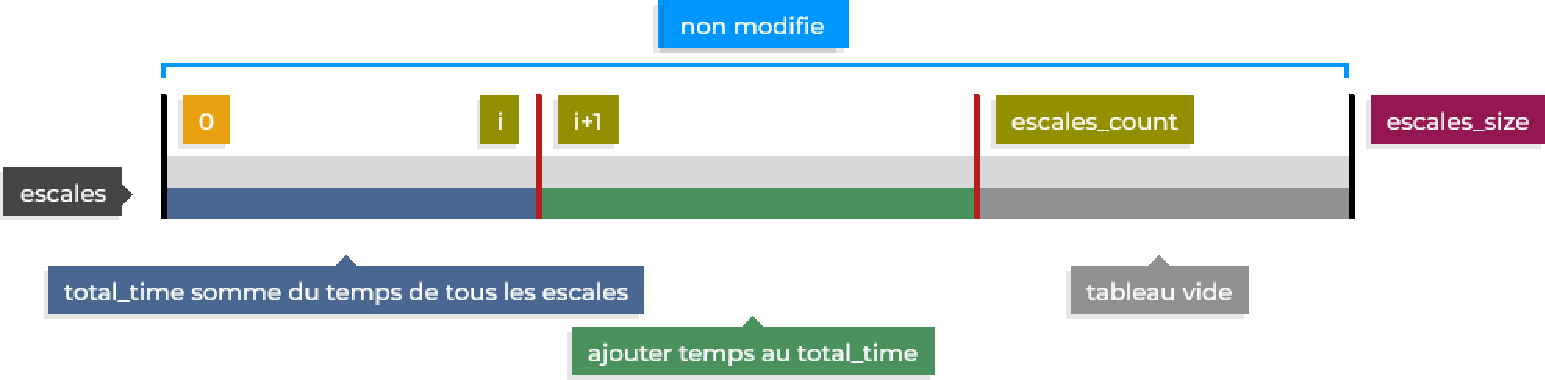
\includegraphics[width=1\textwidth]{invariant_time.pdf}
    \caption{Invariant graphique}
\end{figure}

\textbf{Invariant formel:} \\
    $escale = escale_0$ \\
    $\land$ \\
    $0 < i < escale\_count$ \\
    $\land$ \\
    $total\_time = \sum_{i=0}^{escale\_count-1} \texttt{get\_time}(escales[i])$


% !TEX root = ./main.tex
%%%%%%%%%%%%%%%%%%%%%%%%%%%%%%%%%%%%%%%%%%%%%%%%%%%%%%%%%%%%%%%%%%%%%%%%%%%%%%%%%%%%%%%%%%
% Dans cette section, il est demandé d'appliquer l'approche constructive pour la         %
% construction de votre code.                                                            %
%                                                                                        %
% Pour chaque Sous-Problème (une sous-section/SP):                                       %
% - {Pré} INIT {INV}                                                                     %
% - déterminer le Critère d'Arrêt (et donc le Gardien de Boucle)                         %
% - {INV & B} ITER {INV}                                                                 %
% - {INV & !B} END {Post}                                                                %
% - Fonction de Terminaison (pensez à justifier sur base de l'Invariant Graphique)       %
% (une sous-sous-section/tiret)                                                          %
%%%%%%%%%%%%%%%%%%%%%%%%%%%%%%%%%%%%%%%%%%%%%%%%%%%%%%%%%%%%%%%%%%%%%%%%%%%%%%%%%%%%%%%%%%
\section{Approche Constructive}
%%%%%%%%%%%%%%%%%%%%%%%%%%%%%%%%

\begin{lstlisting}[caption={Un programme tout simple}]
int main(void)
{
    // Les commandes Latex sont permises dans les commentaires sur une ligne. Exemple : $x_i \leq a ^b$
    printf("Bonjour tout le monde !");
    /*
    Dans les commentaires sur plusieurs lignes, elles doivent être entourées
    de symboles définis par l'option « escapeinside » de \lstset
    (>\coms{$\sum_{i = 1}^N 1 = N$}<)
    La commande « \coms » permet de colorer correctement le code latex ajouté.
    Les accents et tous les autres diacritiques sont permis : àÀçÇéÉèÈêÊœŒ...
    */
    return 1; (>\label{code:ret}<)
}
\end{lstlisting}

Il est possible de faire référence à la ligne \ref{code:ret} de l'extrait de code.


% !TEX root = ./main.tex
%%%%%%%%%%%%%%%%%%%%%%%%%%%%%%%%%%%%%%%%%%%%%%%%%%%%%%%%%%%%%%%%%%%%%%%%%%%%%%%%%%%%%%%%%%
% Dans cette section, indiquez le code complet (sans assertions intermédiaires) de votre %
% solution                                                                               %
%%%%%%%%%%%%%%%%%%%%%%%%%%%%%%%%%%%%%%%%%%%%%%%%%%%%%%%%%%%%%%%%%%%%%%%%%%%%%%%%%%%%%%%%%%
\section{Code Complet}\label{code}
%%%%%%%%%%%%%%%%%%%%%%%

\lstinputlisting[caption=Implémentation de prefixe\_suffixe]
    {../code/prefixe_suffixe.c}


% !TEX root = ./main.tex
%%%%%%%%%%%%%%%%%%%%%%%%%%%%%%%%%%%%%%%%%%%%%%%%%%%%%%%%%%%%%%%%%%%%%%%%%%%%%%%%%%%%%%%%%%
% Dans cette section, vous devez étudier complètement la complexité de votre code.       %
% Soyez le plus formel (i.e., mathématique) possible.                                    %
%%%%%%%%%%%%%%%%%%%%%%%%%%%%%%%%%%%%%%%%%%%%%%%%%%%%%%%%%%%%%%%%%%%%%%%%%%%%%%%%%%%%%%%%%%
\section{Complexité}\label{complexite}
%%%%%%%%%%%%%%%%%%%%

\subsection{Fonctions sur Escale}

\begin{itemize}
    \item escale\_create : $\mathcal{O}(1)$
    \item escale\_get\_name : $\mathcal{O}(1)$
    \item escale\_get\_x : $\mathcal{O}(1)$
    \item escale\_get\_y : $\mathcal{O}(1)$
    \item escale\_get\_best\_time : $\mathcal{O}(1)$
    \item escale\_set\_best\_time : $\mathcal{O}(1)$
    \item escale\_distance : $\mathcal{O}(1)$
    \item escale\_equal : $\mathcal{O}(1)$
\end{itemize}

\subsection{Opérations sur Course (tableau dynamique)}
Soit $n$ le nombre d'escales, $S$ la capacité du tableau.

\begin{align*}
&\texttt{course\_append} :
    \begin{cases}
        \mathcal{O}(1) & \text{(amorti)} \\
        \mathcal{O}(n) & \text{(réallocation)}
    \end{cases} \\
&\texttt{course\_pop} : \mathcal{O}(1) \\
&\texttt{course\_get\_escales\_count} : \mathcal{O}(1) \\
&\texttt{course\_total\_time} : \mathcal{O}(n) \\
&\texttt{course\_best\_time\_at}(i) : \mathcal{O}(1) \\
&\text{Espace mémoire} : \mathcal{O}(S),\ S \geq n
\end{align*}

\subsection{Opérations sur \texttt{Course} (liste chaînée)}

Soit $n$ le nombre d'escales.

\begin{align*}
&\texttt{course\_append} : \mathcal{O}(n) \\
&\texttt{course\_pop} : \mathcal{O}(n) \\
&\texttt{course\_get\_escales\_count} : \mathcal{O}(n) \\
&\texttt{course\_total\_time} : \mathcal{O}(n) \\
&\texttt{course\_best\_time\_at}(i) : \mathcal{O}(i) \\
&\texttt{course\_last} : \mathcal{O}(n) \\
&\text{Espace mémoire} : \mathcal{O}(n)
\end{align*}


% !TEX root = ./main.tex
%%%%%%%%%%%%%%%%%%%%%%%%%%%%%%%%%%%%%%%%%%%%%%%%%%%%%%%%%%%%%%%%%%%%%%%%%%%%%%%%%%%%%%%%%%
% Rédigez ici la conclusion de votre rapport.                                            %
%%%%%%%%%%%%%%%%%%%%%%%%%%%%%%%%%%%%%%%%%%%%%%%%%%%%%%%%%%%%%%%%%%%%%%%%%%%%%%%%%%%%%%%%%%
\section{Conclusion}\label{conclusion}
%%%%%%%%%%%%%%%%%%%%%

C'est un cours difficile


%%%%%%%%%%%%%%%%%%%% FIN DE LA ZONE PROTÉGÉE %%%%%%%%%%%%%%%%%%%%

\end{document}
